%  A simple AAU PhD thesis template (collection of papers).
%  2016-08-01 v. 1.3.1
%  Copyright 2012-2016 by Jesper Kjær Nielsen <jkn@es.aau.dk>
%
%  This is free software: you can redistribute it and/or modify
%  it under the terms of the GNU General Public License as published by
%  the Free Software Foundation, either version 3 of the License, or
%  (at your option) any later version.
%
%  This is distributed in the hope that it will be useful,
%  but WITHOUT ANY WARRANTY; without even the implied warranty of
%  MERCHANTABILITY or FITNESS FOR A PARTICULAR PURPOSE.  See the
%  GNU General Public License for more details.
%
%  You can find the GNU General Public License at <http://www.gnu.org/licenses/>.
%
%  A simple AAU PhD thesis template (collection of papers).
%  2016-08-01 v. 1.3.1
%  Copyright 2012-2016 by Jesper Kjær Nielsen <jkn@es.aau.dk>
%
%  This is free software: you can redistribute it and/or modify
%  it under the terms of the GNU General Public License as published by
%  the Free Software Foundation, either version 3 of the License, or
%  (at your option) any later version.
%
%  This is distributed in the hope that it will be useful,
%  but WITHOUT ANY WARRANTY; without even the implied warranty of
%  MERCHANTABILITY or FITNESS FOR A PARTICULAR PURPOSE.  See the
%  GNU General Public License for more details.
%
%  You can find the GNU General Public License at <http://www.gnu.org/licenses/>.
%
\documentclass[10pt,twoside,openright]{book}
%%%%%%%%%%%%%%%%%%%%%%%%%%%%%%%%%%%%%%%%%%%%%%%%
% Language, Encoding and Fonts
% http://en.wikibooks.org/wiki/LaTeX/Internationalization
%%%%%%%%%%%%%%%%%%%%%%%%%%%%%%%%%%%%%%%%%%%%%%%%
% Select encoding of your inputs. Depends on
% your operating system and its default input
% encoding. Typically, you should use
%   Linux  : utf8 (most modern Linux distributions)
%            latin1
%   Windows: ansinew
%            latin1 (works in most cases)
%   Mac    : applemac
% Notice that you can manually change the input
% encoding of your files by selecting "save as"
% an select the desired input encoding.
\usepackage[utf8]{inputenc}
% Make latex understand and use the typographic
% rules of the language used in the document.
\usepackage[danish,english]{babel}
% Use the palatino font
\usepackage[sc]{mathpazo}
\linespread{1.05}         % Palatino needs more leading (space between lines)
\setlength{\parskip}{0.65em}
% Choose the font encoding
% Choose the font encoding
\usepackage[T1]{fontenc}
%%%%%%%%%%%%%%%%%%%%%%%%%%%%%%%%%%%%%%%%%%%%%%%%
% Graphics and Tables
% http://en.wikibooks.org/wiki/LaTeX/Importing_Graphics
% http://en.wikibooks.org/wiki/LaTeX/Tables
% http://en.wikibooks.org/wiki/LaTeX/Colors
%%%%%%%%%%%%%%%%%%%%%%%%%%%%%%%%%%%%%%%%%%%%%%%%
% load a colour package
\usepackage{xcolor}
% UniPrint prefers that no colours are used in the template by default.
% However, if you want some colours, then you can easily change the following
\definecolor{aaublue}{RGB}{0,0,0}% black
%\definecolor{aaublue}{RGB}{33,26,82}% dark blue
% The standard graphics inclusion package
\usepackage{graphicx}
% Set up how figure and table captions are displayed
\usepackage{caption}
\captionsetup{%
  font=footnotesize,% set font size to footnotesize
  labelfont=bf % bold label (e.g., Figure 3.2) font
}
% Make the standard latex tables look so much better
\usepackage{array,booktabs}
\usepackage{tabularx}
\usepackage{multirow}
% Enable the use of frames around, e.g., theorems
% The framed package is used in the example environment
\usepackage{framed}
% Create beautiful plots using TikZ and PGFPLOTS
\usepackage{tikz,pgfplots}
%%%%%%%%%%%%%%%%%%%%%%%%%%%%%%%%%%%%%%%%%%%%%%%%
% Mathematics
% http://en.wikibooks.org/wiki/LaTeX/Mathematics
%%%%%%%%%%%%%%%%%%%%%%%%%%%%%%%%%%%%%%%%%%%%%%%%
% Defines new environments such as equation,
% align and split
\usepackage{amsmath}
% Adds new math symbols
\usepackage{amssymb}
% Use theorems in your document
% The ntheorem package is also used for the example environment
% When using thmmarks, amsmath must be an option as well. Otherwise \eqref doesn't work anymore.
\usepackage[framed,amsmath,amsthm,thmmarks]{ntheorem}

%%%%%%%%%%%%%%%%%%%%%%%%%%%%%%%%%%%%%%%%%%%%%%%%
% Page Layout and appearance
% http://en.wikibooks.org/wiki/LaTeX/Page_Layout
%%%%%%%%%%%%%%%%%%%%%%%%%%%%%%%%%%%%%%%%%%%%%%%%
% Change margins, papersize, etc of the document
\usepackage[
  paperwidth=17cm, % width of a page
  paperheight=24cm, % height of a page
  outer=2.5cm, % right margin on an odd page
  inner=2.5cm, % left margin on an odd page
  top=2.5cm, % top margin
  bottom=2.5cm % bottom margin
  ]{geometry}
% Enable the crop package if you want to print on a4 paer
%\usepackage[a4,cam,center]{crop}
% Modify how \chapter, \section, etc. look
\renewcommand{\thesection}{\arabic{section}}
% The titlesec package is very configureable
\usepackage{titlesec}
\titleformat*{\section}{\normalfont\Large\bfseries\color{aaublue}}
\titleformat*{\subsection}{\normalfont\large\bfseries\color{aaublue}}
\titleformat*{\subsubsection}{\normalfont\normalsize\bfseries\color{aaublue}}
%\titleformat*{\paragraph}{\normalfont\normalsize\bfseries\color{aaublue}}
%\titleformat*{\subparagraph}{\normalfont\normalsize\bfseries\color{aaublue}}
% Change some default names
\addto\captionsenglish{%this line is required when using the babel package
  \renewcommand\appendixname{Paper} % change Appendix to Paper
  \renewcommand\bibname{References} % change Bibliography to references
  \renewcommand\figurename{Fig.} % change Figure to Fig.
}

% Change the headers and footers
\usepackage{fancyhdr}
\pagestyle{fancy}
\fancyhf{} %delete everything
\renewcommand{\headrulewidth}{0pt} %remove the horizontal line in the header
\fancyhead[CE]{\color{aaublue}\small\nouppercase\leftmark} %even page - chapter title
\fancyhead[CO]{\color{aaublue}\small\nouppercase\rightmark} %uneven page - section title
\fancyfoot[CE,CO]{\thepage} %page number on all pages
% Do not stretch the content of a page. Instead,
% insert white space at the bottom of the page
\raggedbottom
% Enable arithmetics with length. Useful when
% typesetting the layout.
\usepackage{calc}
% fix the marginpar command so it is always on the correct side
\usepackage{mparhack}

%%%%%%%%%%%%%%%%%%%%%%%%%%%%%%%%%%%%%%%%%%%%%%%%
% Bibliography
% http://en.wikibooks.org/wiki/LaTeX/Bibliography_Management
%%%%%%%%%%%%%%%%%%%%%%%%%%%%%%%%%%%%%%%%%%%%%%%%
% Bibliography for each chapter
\usepackage[sectionbib]{chapterbib}
% Custom bibliograhy - used in the list of papers
%\usepackage{multibib}
%\newcites{main}{Main References}
%\newcites{other}{Other Publications}
% Change [1,2,3,4] into [1-4]
\usepackage{cite}

%%%%%%%%%%%%%%%%%%%%%%%%%%%%%%%%%%%%%%%%%%%%%%%%
% Misc
%%%%%%%%%%%%%%%%%%%%%%%%%%%%%%%%%%%%%%%%%%%%%%%%
% Add bibliography and index to the table of
% contents
\usepackage[nottoc,section]{tocbibind}
% Enable subappendices
\usepackage{appendix}
\renewcommand{\setthesection}{\Alph{section}} % remove the chapter numbering
% Add the command \pageref{LastPage} which refers to the
% page number of the last page
\usepackage{lastpage}
% Add notes to in your document
\usepackage[
%  disable, %turn off todonotes
  colorinlistoftodos, %enable a coloured square in the list of todos
  textwidth=2cm, %set the width of the todonotes
  textsize=scriptsize, %size of the text in the todonotes
  ]{todonotes}
\setlength{\marginparwidth}{2cm}

%%%%%%%%%%%%%%%%%%%%%%%%%%%%%%%%%%%%%%%%%%%%%%%%
% Hyperlinks
% http://en.wikibooks.org/wiki/LaTeX/Hyperlinks
%%%%%%%%%%%%%%%%%%%%%%%%%%%%%%%%%%%%%%%%%%%%%%%%
% Enable hyperlinks and insert info into the pdf
% file. Hypperref should be loaded as one of the
% last packages
\usepackage{hyperref}
\hypersetup{%
	pdfpagelabels=true,%
	plainpages=false,%
	pdfauthor={Author},%
	pdftitle={Title},%
	pdfsubject={Subject},%
	bookmarksnumbered=true,%
	colorlinks=true,%
	citecolor=aaublue,%
	filecolor=aaublue,%
	linkcolor=aaublue,% you should probably change this to black before printing
	urlcolor=aaublue,%
	pdfstartview=FitH%
}

%%%%%%%%%%%%%%%%%%%%%%%%%%%%%%%%%%%%%%%%%%%%%%%%
% My included packages
%%%%%%%%%%%%%%%%%%%%%%%%%%%%%%%%%%%%%%%%%%%%%%%%
% pdfpages: For including the papers that I need
\usepackage[final]{pdfpages}

% acronym: For including the acronyms used in the thesis manuscript
%\usepackage[nolist]{acronym} -> To not include the file list.
\usepackage{acronym} % Include the list of acronyms in the output file

% array: for table values centering
\usepackage{array}
\newcolumntype{P}[1]{>{\centering\arraybackslash}p{#1}}
\newcolumntype{M}[1]{>{\centering\arraybackslash}m{#1}}
% package inclusion and set up of the document
% see, e.g., http://en.wikibooks.org/wiki/LaTeX/Formatting#Hyphenation
% for more information on word hyphenation
\hyphenation{ex-am-ple hy-phen-a-tion short}
\hyphenation{long la-tex}
%
%  A simple AAU PhD thesis template (collection of papers).
%  2016-08-01 v. 1.3.1
%  Copyright 2012-2016 by Jesper Kjær Nielsen <jkn@es.aau.dk>
%
%  This is free software: you can redistribute it and/or modify
%  it under the terms of the GNU General Public License as published by
%  the Free Software Foundation, either version 3 of the License, or
%  (at your option) any later version.
%
%  This is distributed in the hope that it will be useful,
%  but WITHOUT ANY WARRANTY; without even the implied warranty of
%  MERCHANTABILITY or FITNESS FOR A PARTICULAR PURPOSE.  See the
%  GNU General Public License for more details.
%
%  You can find the GNU General Public License at <http://www.gnu.org/licenses/>.
%
%
%
% see, e.g., http://en.wikibooks.org/wiki/LaTeX/Customizing_LaTeX#New_commands
% for more information on how to create macros

%%%%%%%%%%%%%%%%%%%%%%%%%%%%%%%%%%%%%%%%%%%%%%%%
% Environment
%%%%%%%%%%%%%%%%%%%%%%%%%%%%%%%%%%%%%%%%%%%%%%%%
%example
\theoremheaderfont{\normalfont\bfseries}
\theorembodyfont{\normalfont}
\theoremstyle{break}
\def\theoremframecommand{{\color{aaublue!50}\vrule width 5pt \hspace{5pt}}}
\newshadedtheorem{exa}{Example}[section]
\newenvironment{example}[1]{%
		\begin{exa}[#1]
}{%
		\end{exa}
}

%assumptions
\newtheorem{ass}{Assumption}[section] % assumptions

%%%%%%%%%%%%%%%%%%%%%%%%%%%%%%%%%%%%%%%%%%%%%%%%
% Paper Inclusion
%%%%%%%%%%%%%%%%%%%%%%%%%%%%%%%%%%%%%%%%%%%%%%%%
% include a paper
\newcommand{\includepaper}[1]{
  \cleardoublepage
  \setcounter{enumiii}{0}
  \setcounter{enumii}{0}
  \setcounter{enumiv}{0}
  \setcounter{enumi}{0}
  \setcounter{equation}{0}
  \setcounter{figure}{0}
  \setcounter{footnote}{0}
%  \setcounter{lofdepth}{1}
%  \setcounter{lotdepth}{1}
  \setcounter{mpfootnote}{0}
  \setcounter{paragraph}{0}
  \setcounter{parentequation}{0}
  \setcounter{part}{0}
  \setcounter{section}{0}
%  \setcounter{subfigure}{0}
  \setcounter{subparagraph}{0}
  \setcounter{subsection}{0}
  \setcounter{subsubsection}{0}
%  \setcounter{subtable}{0}
  \setcounter{table}{0}
  \include{#1}
}

% create the paper titlepage
\newcommand{\papertitlepage}[5]{
  \chapter{#1}\label{#2}
  \chaptermark{}
  \vspace{2cm}
  \begin{center}
    \large #3
  \end{center}
  \vspace{3cm}
  \begin{center}
  \normalsize #4
  \end{center}
  \vspace*{\fill}
  \newpage\thispagestyle{empty}
  \vspace*{\fill}
    #5\par
    \noindent{\em The layout has been revised.}
  \vspace*{\fill}
  \cleardoublepage
}

% environment for abstracts
\newenvironment{abstract}{\section*{Abstract}\it}{}


%%%%%%%%%%%%%%%%%%%%%%%%%%%%%%%%%%%%%%%%%%%%%%%%
% Various names
%%%%%%%%%%%%%%%%%%%%%%%%%%%%%%%%%%%%%%%%%%%%%%%%
\newcommand{\IEEEPARstart}[2]{#1#2}


%%%%%%%%%%%%%%%%%%%%%%%%%%%%%%%%%%%%%%%%%%%%%%%%
% Bibliography
%%%%%%%%%%%%%%%%%%%%%%%%%%%%%%%%%%%%%%%%%%%%%%%%
\newcommand{\defaultbib}{%
  \bibliographystyle{IEEEtran}
  \bibliography{bib/mybib}
}
% my new macros

\begin{document}
%frontmatter
\frontmatter
\pagestyle{empty} %disable headers and footers
\pagenumbering{roman} %use roman page numbering in the frontmatter
%  A simple AAU PhD thesis template (collection of papers).
%  2016-08-01 v. 1.3.1
%  Copyright 2012-2016 by Jesper Kjær Nielsen <jkn@es.aau.dk>
%
%  This is free software: you can redistribute it and/or modify
%  it under the terms of the GNU General Public License as published by
%  the Free Software Foundation, either version 3 of the License, or
%  (at your option) any later version.
%
%  This is distributed in the hope that it will be useful,
%  but WITHOUT ANY WARRANTY; without even the implied warranty of
%  MERCHANTABILITY or FITNESS FOR A PARTICULAR PURPOSE.  See the
%  GNU General Public License for more details.
%
%  You can find the GNU General Public License at <http://www.gnu.org/licenses/>.
%
\pdfbookmark[0]{Front page}{label:frontpage}%
\begin{titlepage}
  \addtolength{\hoffset}{0.5\evensidemargin-0.5\oddsidemargin} %set equal margins on the frontpage - remove this line if you want default margins
  \noindent%
  \begin{tabular}{@{}p{\textwidth}@{}}
    \toprule[2pt]
    \midrule
    \vspace{0.2cm}
    \begin{center}
    \Huge{\textbf{
      Network Coding\\for Cooperation in\\Wireless Networks
    }} % insert your title here
    \end{center}
    \vspace{0.2cm}\\
    \midrule
    \toprule[2pt]
  \end{tabular}
  \vspace{4 cm}
  \begin{center}
    {\large
      Ph.D. Dissertation%Insert document type (e.g., Project Report)
    }\\
    \vspace{0.2cm}
    {\Large
      N\'estor Javier Hern\'andez Marcano
    }%Insert your group name or real names
  \end{center}
  \vfill
  \begin{center}
  Dissertation submitted October 15, 2016
  \end{center}
\end{titlepage}
\clearpage

\thispagestyle{empty}
\noindent
\begin{tabularx}{\textwidth}{@{}lX}
    Thesis submitted: & Month XX, 20XX\\
    PhD Supervisor: & Prof.\ XX\\
                    & Aalborg University\\
    Assistant PhD Supervisor: & Assoc.\ Prof.\ XX\\
                    & Aalborg University\\
    PhD Committee: & Prof.\ X, Y University\\
                   & Prof.\ X, Y University\\
                   & Prof.\ X, Y University\\
    PhD Series:    & Faculty of X, Aalborg University\\
\end{tabularx}
\strut\vfill
\noindent
\begin{tabularx}{\textwidth}{@{}lX}
    ISSN: & xxxx-xxxx\\
    ISBN: & xxx-xx-xxxx-xxx-x\\
\end{tabularx}
\strut\vfill
\noindent Published by:\newline
Aalborg University Press\newline
Skjernvej 4A, 2nd floor\newline
DK – 9220 Aalborg Ø\newline
Phone: +45 99407140\newline
aauf@forlag.aau.dk\newline
forlag.aau.dk
\strut\vfill
\noindent \copyright{} Copyright by author\newline
\strut\vfill
\noindent Printed in Denmark by Rosendahls, 20XX
\strut\vfill\vfill\vfill
\noindent Normalsider: XXX sider (á 2.400 anslag inkl. mellemrum).\\
Standard pages: XXX pages (2,400 characters incl. spaces).
\clearpage


%% mainfile: ../master.tex
\chapter*{Curriculum Vitae\markboth{Curriculum Vitae}{Curriculum Vitae}}\label{ch:cv}
\pagestyle{fancy}
\addcontentsline{toc}{chapter}{Curriculum Vitae}
\begin{tabularx}{\textwidth}{@{}Xr}
    \Large Author name & \raisebox{-\totalheight/2}{
\includegraphics[width=2cm]{frontmatter/cvPicture.png}}\\
\end{tabularx}\par
\vspace{0.5cm}\noindent
Here is the CV text.

% mainfile: ../master.tex
\chapter*{Abstract\markboth{Abstract}{Abstract}}\label{ch:Abstract}
\addcontentsline{toc}{chapter}{Abstract}

Communication technologies through wireless networks generate today a large demand in high-quality data services that is only expected to grow dramatically in the following years. This future demand will saturate the networks as we know them today. Therefore, This becomes critical in scenarios with a very high density of users, e.g. sports stadiums, where the radio resources are insufficient to deliver a good \ac{QoE}. Thus, exploiting techniques that better use the available resources by exploiting short-range communication alternatives, e.g. \ac{WiFi}, \ac{D2D} in \ac{LTE-A}, to allow cooperation between users is at the crux of delivering the necessary \ac{QoE}. In this scenario, mobile devices with any of the previous short-range communication technologies can cooperate by forming \textit{mobile clouds}. These are cluster of devices exploiting a much faster and reliable communications channel to share information. \ac{NC} has proven to be an effective solution to this scenario since it avoids processing delays from state of the art erasure correcting codes when doing multihop communications.

In this thesis we focused on the design, analysis and simulation of cooperation techniques based on \ac{RLNC} for wireless networks. First, we investigated the operational regimes where cooperative cellular networks perform better than broadcast cellulars networks in terms of data rate and energy costs and also by considering different amount of devices cooperation. Further, we reviewed code constructions that are optimal in other key performance metrics such as total overhead. These works indicate when and how to cooperate between the devices to offload the network, while keeping a minimum overhead Second, we evaluated transmission policies and \ac{MAC} mechanisms to reduce the energy consumption at the devices and increase the throughput in decentralized in \ac{WLAN}. Here, we developed a software framework to perform our analysis using the ns-3 simulator that is publicly available to the research community as a major contribution and showed the possibility to analyze heuristics in an easy fashion. Overall, our techniques address key challenges in state of the art wireless networks to cope with future demands in a satisfactory manner for operator and end-users.


\chapter*{Resumé\markboth{Resumé}{Resumé}}\label{ch:Resume}
\addcontentsline{toc}{chapter}{Resumé}
Danish Abstract

\chapter*{Thesis Details\markboth{Thesis Details}{Thesis Details}}\label{ch:theis_details}
\addcontentsline{toc}{chapter}{Thesis Details}

%this is a mandatory page. You can see more at http://www.phd.teknat.aau.dk/intranet/templates/
\begin{tabularx}{\textwidth}{@{}>{\bfseries}l X@{}}
  Thesis Title: & Network Coding for Cooperation in Wireless Networks\\
  Ph.D. Student: & N\'estor Javier Hern\'andez Marcano\\
  Supervisors: & Assoc.\ Prof.\ Daniel R. Lucani, Aalborg University\\
               & Dr. Janus Heide, Steinwurf ApS\\
               & Prof.\ Frank H.P. Fitzek, Technische Universit\"{a}t Dresden\\
\end{tabularx}
\vspace{\baselineskip}

% list the papers included in this thesis
\noindent The main body of this thesis consist of the following papers:
\begin{itemize}

  \item[{[\ref{paper:paperA}]}] N\'estor J. Hern\'andez Marcano, Janus Heide, Daniel E. Lucani, Frank H.P. Fitzek, ``On the Throughput and Energy Benefits of Network Coded Cooperation'', \emph{2014 IEEE 3rd International Conference on Cloud Networking (IEEE Cloudnet)}, pp. 138--142, 2014.

  \item[{[\ref{paper:paperB}]}] N\'estor J. Hern\'andez Marcano, Janus Heide, Daniel E. Lucani, Frank H.P. Fitzek, ``Throughput, Energy and Overhead of Multicast Device-to-Device Communications with Network Coded Cooperation'', \emph{Wiley Transactions on Emerging Telecommunications Technologies  (former European Transactions on Telecommunications). Special Issue: Emerging Topics in Device to Device Communications as Enabling Technology for 5G Systems}, pp. 1--17, 2016.

  \item[{[\ref{paper:paperC}]}] N\'estor J. Hern\'andez Marcano, P\'eter Vingelmann, Morten V. Pedersen, Janus Heide, Daniel E. Lucani, Frank H.P. Fitzek, ``Getting Kodo: Network Coding for the ns-3 Simulator'', \emph{ACM The Workshop in ns-3 (WNS3)}, pp. 101--107, 2016.

  \item[{[\ref{paper:paperD}]}] N\'estor J. Hern\'andez Marcano, Janus Heide, Daniel E. Lucani, Frank H.P. Fitzek, ``On Transmission Policies for Multihop Device-to-Device Communications with Network Coded Cooperation'', \emph{IEEE 22th International Conference on European Wireless}, pp. 350--354, 2016.

\end{itemize}

% Optionally, you can also list other publications, you have been invovled with
\noindent In addition to the main papers, the following publications have also been made:
\begin{itemize}

  \item[\#{[1]}] N\'estor J. Hern\'andez Marcano, Janus Heide, Daniel E. Lucani, Frank H.P. Fitzek, ``On the Overhead of Telescopic Codes in Network Coded Cooperation'', \emph{IEEE 3rd International Conference on Cloud Networking (IEEE Cloudnet)}, pp. 1--6, 2015.

  \item[\#{[2]}] N\'estor J. Hern\'andez Marcano, Jeppe Pihl, Janus Heide, Jeppe Krigslund, P\'eter Vingelmann, Morten V. Pedersen, Daniel E. Lucani, Frank H.P. Fitzek, ``Wurf.it: A Network Coding Reliable Multicast Streaming Solution - NS-3 Simulations and Implementation'', \emph{ACM The Workshop in ns-3: Posters, Demos and Short-Talks Session (WNS3)}, Available online at the ns-3 website: https://www.nsnam.org/workshops/wns3-2016/posters/hernandez-demo-paper.pdf, 2016.

  \item[\#{[3]}] N\'estor J. Hern\'andez Marcano, Chres W. S\o rensen, Juan A. Cabrera Guerrero, Simon Wunderlich, Daniel E. Lucani, Frank H.P. Fitzek, ``On Goodput and Energy Measurements of Network Coding Schemes in the Raspberry Pi'' \emph{MDPI, Journal of Electronics. Special Issue for the Raspberry Pi (Indexed by Elsevier Scopus and Thomson-Reuters ESCI Web of Science)}, 5(4), 66, pp. 1-27, 2016.

  \item[\#{[4]}] Chres W. S\o rensen, N\'estor J. Hern\'andez Marcano, Juan A. Cabrera Guerrero, Simon Wunderlich, Daniel E. Lucani, Frank H.P. Fitzek, ``Easy as Pi: A Network Coding Raspberry Pi Testbed'' \emph{Accepted to MDPI, Journal of Electronics. Special Issue for the Raspberry Pi (Indexed by Elsevier Scopus and Thomson-Reuters ESCI Web of Science)}, 5(4), 67, pp. 1-25, 2016.

  \item[\#{[5]}] N\'estor J. Hern\'andez Marcano, Wei Lu, Ricardo Bassoli, Marco Di Renzo, Daniel E. Lucani ``A Stochastic Geometry Analysis of Broadcast Cellular Networks with Random Linear Network Coding'' \emph{In preparation}.

\end{itemize}

\noindent This thesis has been submitted for assessment in partial fulfillment of the PhD degree. The thesis is based on the submitted or published scientific papers which are listed above. Parts of the papers are used directly or indirectly in the extended summary of the thesis. As part of the assessment, co-author statements have been made available to the assessment committee and are also available at the Faculty. The thesis is not in its present form acceptable for open publication but only in limited and closed circulation as copyright may not be ensured.
\cleardoublepage
\pdfbookmark[0]{Contents}{label:contents}
\pagestyle{fancy} %enable headers and footers again
\tableofcontents
%\listoftodos
% mainfile: ../master.tex
\chapter*{Preface\markboth{Preface}{Preface}}\label{ch:preface}
\pagestyle{fancy}
\addcontentsline{toc}{chapter}{Preface}
Here is the preface

\vfill
\hfill Name

\hfill Aalborg University, \today

% mainfile: ../master.tex
\chapter*{Acknowledgments\markboth{Acknowledgments}{Acknowledgments}}\label{ch:acknowledgments}
\pagestyle{fancy}
\addcontentsline{toc}{chapter}{Acknowledgments}

The experiences during the PhD path of the last three years have been incredible and very enriching both at a personal and a technical level.

\vfill
\hfill N\'estor J. Hern\'andez Marcano

\hfill Aalborg University, \today
\cleardoublepage

%mainmatter
\mainmatter
\part{Introduction}
\newcommand{\introtitle}{Introduction}
\chapter*{\introtitle}\label{sec:intro}
\addcontentsline{toc}{chapter}{\introtitle}

\section{Background}\label{sec:background}
% General introduction
Data demand is predicted to growth by a factor of 10 in 2020 from today values by major network providers \cite{cisco2016forecast,kremling2015presentation,belllabs2016report,ericsson2015report}. The use of cellular networks for data consumption has become
widespread due in part to the massive increase in applications and services for content delivery (Netflix, etc.), social networking (Facebook, Twitter, Snapchat, Instagram, etc.), cloud computing and storage (Dropbox, OneDrive, Amazon S3, Amazon EC2, etc.). Further, content delivery networks will be carrying three-fourths of all the Internet video traffic by the end of 2020 \cite{cisco2016forecast}. Streaming applications that are based in multicast where a transmitter needs to serve tens, hundreds or even thousands of receivers are drawing large attention in mobile networks such as \ac{LTE-A} or \ac{WLAN} networks such as \ac{WiFi}. Use cases of video streaming in highly-crowded scenarios such as sports stadiums, airports, service-waiting areas or museums are attractive to the content providers. These types of scenarios pose tight requirements to ensure a satisfactoring \ac{QoE} for all the customers. First, video services require high throughput and low delay to avoid stalling events in the end-user device. Second, to cope with the users data load, a high-capacity access network is required to accomodate all the users. Third, an efficient transmission schemes are required to serve them as quick as possible. To address these requirements, service providers utilize 4G high-capacity mobile networks or \ac{WiFi} networks using a broadcast schemes to serve all the users.

For the network operator, techniques that can offload the service infrastructure to cope with such control and data load are needed in order to satisfy the overall demand and reduce its energy consumption. Further, given that not all the end-users present similar channel conditions, there might exist users with a degraded connection to a \ac{BS} thus wasting network capacity. Instead, a better connectivity might be provided by other users either within the cellular spectrum or through a \ac{WiFi} network. The management of mobile devices without good cellular coverage but with access to this local network can potentially be decentralized.

For the mobile user, due to data transmissions, device internal energy consumption has become a limiting factor in terms of battery life. Without a transmission scheme properly designed, energy consumed by data transmissions can drain the mobile device battery affecting the user perception of quality in a given service. Besides data transmissions, mobile devices perform much more internal tasks than older devices from ten years ago and since energy has become critical for the users.

Therefore, mobile network designers need to consider mechanisms and techniques that aim for high throughput and low energy consumption both at the station and the end user devices and that are able to provide data offloading from current network infrastructures. An effective solution to this problem is to consider cooperation between the devices. This approach exploits the short-range communications between the mobile devices to offload the network and improve the mentioned metrics.

\subsection{Cooperative Wireless Networks}
% Cooperation
The concept of cooperation in wireless networks has been investigated before \cite{fitzek2006cooperation,fitzek2007cognitive,fitzek2013mobile}. The main goal is to diminish the amount of communications resources (data rate, energy or even storage and computational power) to convey an information of common interest from a transmitter to a set of interconnected receivers in a multicast fashion. Devices connected in this way form a \textit{mobile cloud} \cite{fitzek2013mobile}. In Fig.~\ref{fig:cooperation}, it can be observed a comparison example of no cooperation and cooperation in a multicast wireless network.

\begin{figure}[ht!]
  \centering
  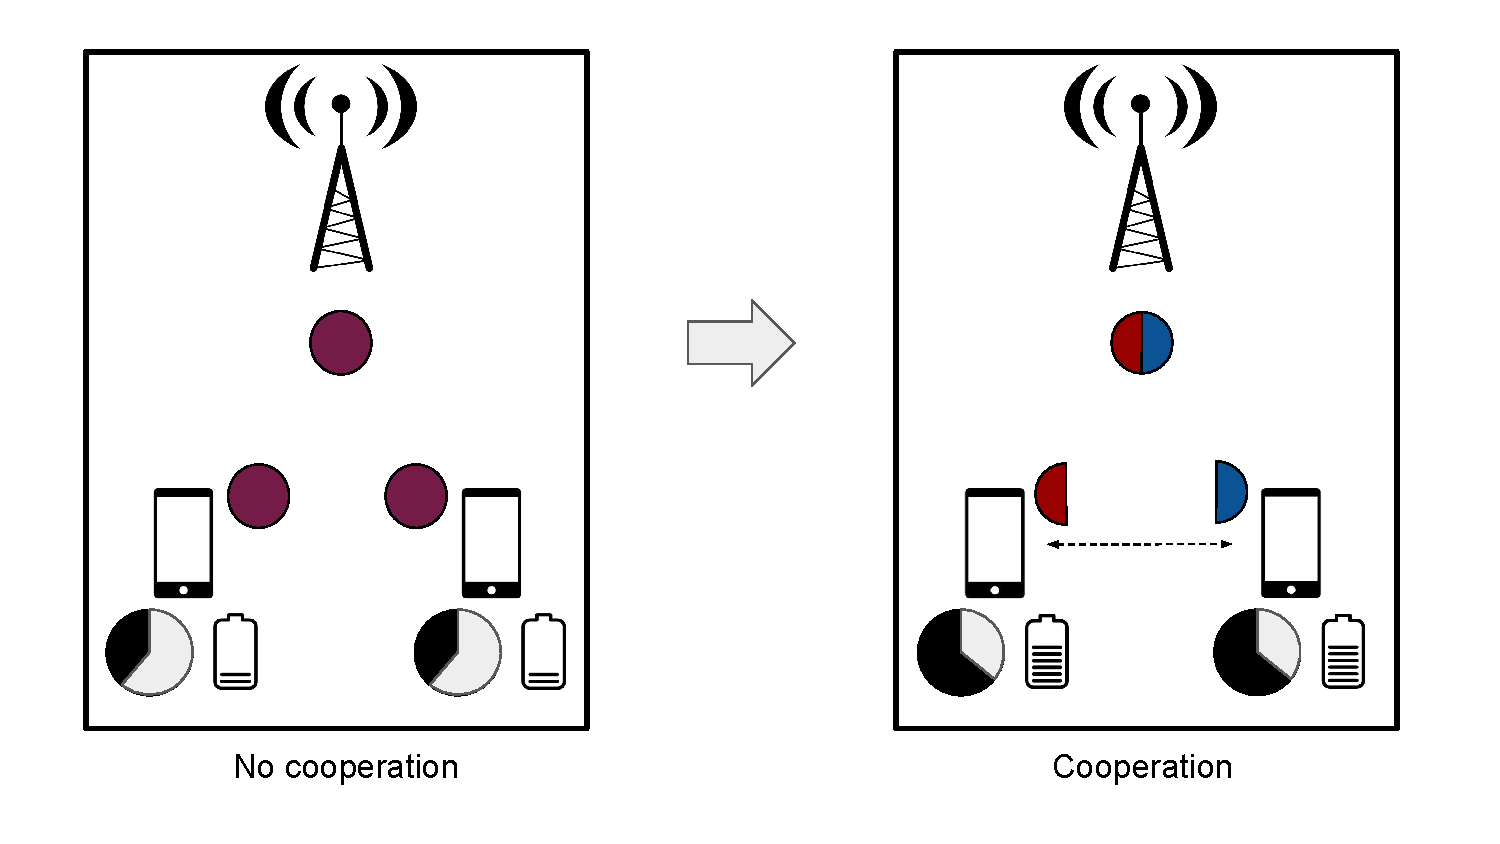
\includegraphics[width=\textwidth]{introduction/figures/cooperation.pdf}
  \caption{Cooperation in Wireless Networks.}
\label{fig:cooperation}
\end{figure}

Without cooperation, a purple content is sent to two mobile devices in a broadcast fashion. This incurs in posible a large downloading time to ensure both devices are satisfied reducing the throughput and increasing the energy consumption.  When cooperation is considered, the content now is split into smaller blue and red pieces where each of them is sent rapidly to each device. Then, the devices exploit short-range communications (dashed line) by exchanging their missing pieces. The key underlying idea is for the devices share their missing information through a faster, short-distance and reliable link which increases the total throughput and reduces the overal energy consumption. From an operator perspective, the information \textit{as a whole} is quickly disseminated into the receivers helping the \ac{BS} to offload data. At the end, the goal of reducing the use communication resources is achieved. In this way, mobile clouds allow to improve the overall network performance and user experience.

\subsection{Device to Device Communications in Mobile Networks}
\label{sec:d2d}
One of the key aspects to achieve the gains proposed by the cooperative approach is the short-range technology to be considered and its parameters to guarantee a fast and reliable link. Besides \ac{WLAN} technologies like \ac{WiFi}, there has been a large interest in \ac{D2D} communications \cite{lin2013comprehensive,asadi2014survey,feng2014device,tehrani2014device}. This permits the devices to share data without going through the \ac{BS} network which keeps the idea of data offloading. The work in \cite{asadi2014survey} proposes a classification of \ac{D2D} communications.

First, according to its spectrum use, the communications could be in the cellular network (inband) or outside in a local network (outband). Second, for inband \ac{D2D} the communications could take place in the spectrum of other mobile users (underlay) or another dedicated only to \ac{D2D} (overlay). Second, for outband \ac{D2D}, the coordination between cellular and local network radio interfaces is either controlled by the cellular \ac{BS} (controlled) or the users themselves (autonomous).

For network assisted or inband \ac{D2D}, authors in \cite{fodor2014design} review the key challenges to enable \ac{D2D} services. Device discovery, communication resource allocation and coordination for these type of communications are handled by the cellular network. Furthermore, \ac{D2D} based \ac{ProSe} have been included in \cite{3gpp2012prose} to use them in \ac{LTE-A} networks for an improved \ac{QoE}.

\subsection{Erasure Correcting Codes for Multicast Networks}
\label{sec:erasure_codes}
Another aspect that is relevant for cooperation gains in multicast scenarios is channel coding. The dynamics of the wireless medium, propagation conditions, noise and interference may degradate the received \ac{SINR} thus making reception unfeasible for some period of time. In the case of packet networks, this leads to \textit{erasure} channels where packets are either correctly received or lost. Therefore, to protect against packet erasures, some redundancy is added through channel coding with a \ac{FEC} technique also called an erasure correcting code. These techniques are relevant to make multicast applications reliable since feedback control through \ac{ACK} packets is not possible for a large number of devices.

Different erasure correcting codes might be used for reliable multicast applications. In the literature, we can find linear block codes such as \ac{RS} \cite{reed1960polynomial} or \ac{LDPC} \cite{gallager1962low}. More recently, \ac{LT} codes \cite{luby2002lt} and Raptor codes \cite{shokrollahi2006raptor} are codes that are more adaptable to the channel conditions than block codes. These latter type of codes are characterized by being: (i) Able to generate a very large number of coded symbols, i.e. rateless, (ii) close-to-optimal, i.e requiring a slightly higher amount of encoded symbols than the original set to decode and (iii) able to decode with a subset of coded symbols as long as there are no inter-dependencies in it. These erasure correction properties among others have led to consider Raptor codes for its standardization in multicast \ac{LTE-A} networks through the \ac{eMBMS} protocol \cite{embms2014general}.

Although these coding techniques are useful for multicast networks, they pose two major restrictions to apply them with the cooperative approach. First, this type of coding is made on a \textit{link} basis, meaning that for each hop encoding and decoding needs to take place. The required code processing for each hop brings delays and energy consumption due to computational aspects \cite{toemoeskoezi2015packet}. Second, as a consequence of the previous, these codes are not composable in principle. This implies that there are no known forms to create new coded packets from packets that have been coded previously without decoding in the case of rateless codes. Because of these limitations state of the art rateless codes are not ideal erasure correcting codes for cooperative wireless networks with \ac{D2D} due to the inherent processing in multihop.

\subsection{Intra-Session Network Coding for Multicast Networks}
% Network Coding, inter-session (XOR) and intra-session (RLNC)
Introduced by Alshwede et al. \cite{ahlswede2000network}, \ac{NC} appeared as an effective technology to remove the limitations presented previously. In this work, the authors presented a new paradigm shift for conveying information in communication networks. Instead of treating the packets as atomic, unmodifiable units at the intermediates node in a network, they are regarded as algebraic elements in a \ac{GF} that can be operated on to create new coded packets. In \cite{ahlswede2000network}, the authors considered the binary field to perform the algebraic operations. This type of coding became known later as inter-session network coding since packets from two sessions where mixed in the coding process. Due to the binary field nature, it also became known as XOR coding since this operation is congruent with the modulo-2 addition. However, limitation for this coding scheme is that specific topologies needs to occur for taking advantage of the codes which might not be the case in our scenarios.

Besides inter-session network coding, intra-session network coding known as \ac{RLNC} \cite{ho2006random}, was introduced by Ho et al. Here, coded packets are algebraic linear combinations of original set of packets from a single data flow. This removes the limitation of sending \textit{particular} packets by now sending coded packets as linear equations of the originals. Given that packets are mixed from a single flow, there are no requirements for a specific topology to use \ac{RLNC}. This type of coding can be made across any node in the network. Further, \ac{RLNC} is proven to achieve the multicast capacity from a flow perspective with very high probability \cite{koetter2003algebraic,ho2006random}. In this way, instead of typically encoding and decoding on a hop basis, coding is made on a \textit{network} basis. Relaying nodes can recode packets to reduce delay and still take advantage of the data representation for the next hop. In this sense, \ac{RLNC} appears as the only coding technique that overcomes the restrictions mentioned earlier in Section~\ref{sec:erasure_codes}.

\begin{figure}[h]
  \centering
  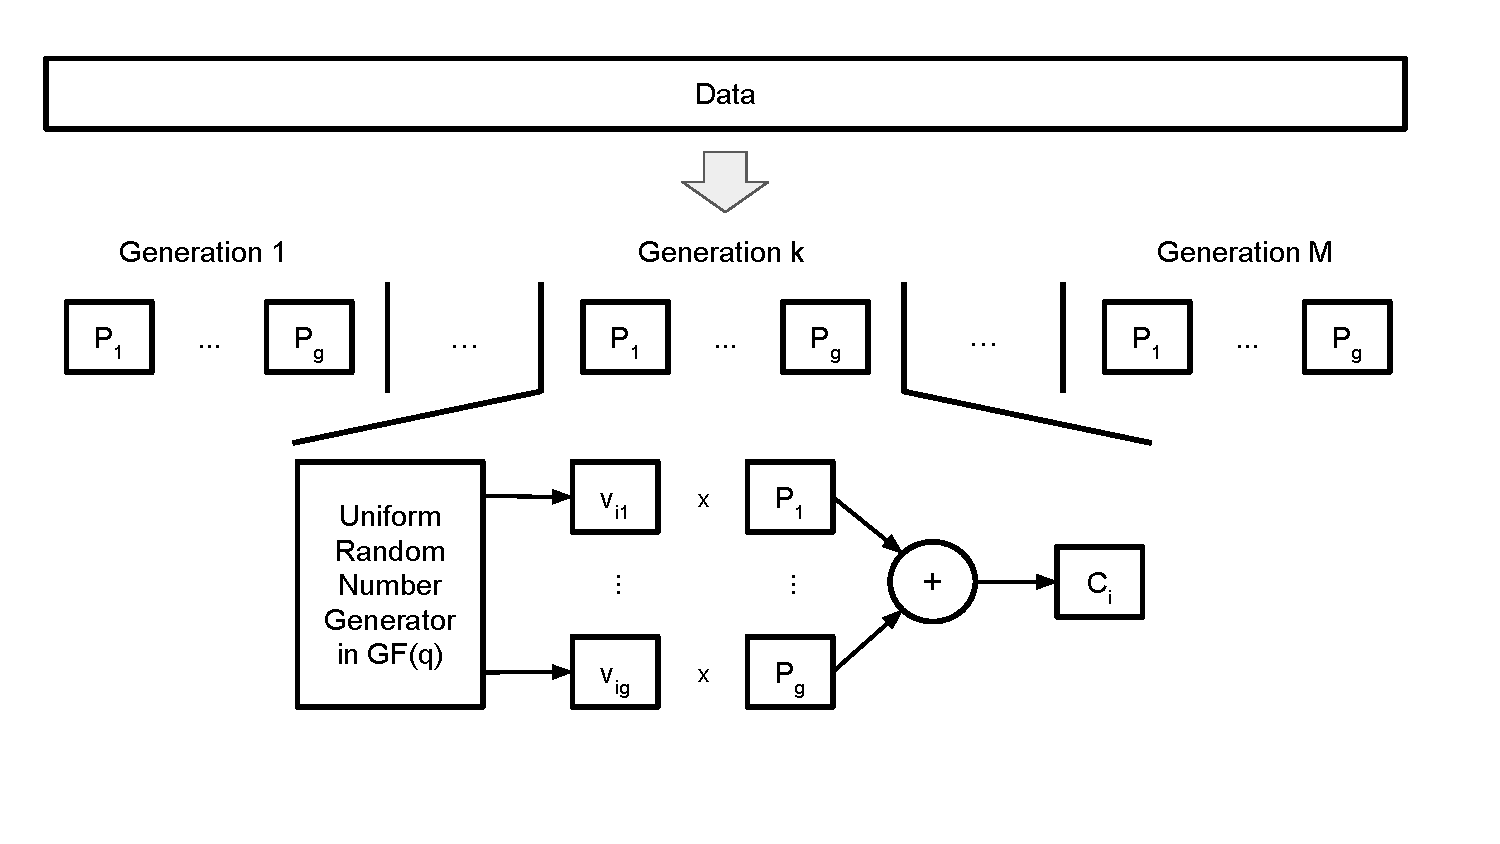
\includegraphics[width=\textwidth]{introduction/figures/RLNC.pdf}
  \caption{RLNC encoding process.}
\label{fig:rlnc_enc}
\end{figure}

As seen in Fig.~\ref{fig:rlnc_enc}, in \ac{RLNC} the information to be transmitted is split into packets which are grouped into sets called \textit{generations} \cite{chou2003practical}. Each generation $k = 1, \ldots, M$ consists of $g$ original packets $P_i,\ i = 1, \ldots, g$ used to create new coded packets as with any \ac{FEC} technique from Section~\ref{sec:erasure_codes}. For each generation, each coded packet generated is a linear combination of all the original packets $C_i = \sum_{j = 1}^g v_{ij} P_i,\ i \geq 1$. Here, $v_{ij}$ is the coding coefficient that multiplies packet $j$ in the process of creating packet $i$. The coefficients are picked uniformly at random from $GF(q)$ where $q$ is the field size. All the operations are properly defined under the arithmetics of $GF(q)$.

After creating a coded packet, it is necessary to signal the coding coefficients utilized for encoding to the decoder. The signalling method that guarantees potential recoding without major caveats, is to append each coding coefficient used to create that coded packet as overhead. For each coded packet there is an overhead of $|v_{ij}| = \sum_{j = 1}^g \log_{2}(q) = g \times \log_{2}(q),\ \forall i,j$ bits. To get the original packets, a decoder only needs to collect \textit{any} set of $g$ linearly independent coded packets to create a $g \times g$ matrix with the coding coefficients and perform Gaussian elimination \cite{fragouli2006network} to solve the linear equations made in the encoding process.

Despite being a relatively recent technology, practical applications of \ac{RLNC} started to appear a few years after its inception. The work of Chachulski et al. in 2007 considered \ac{MORE} \cite{chachulski2007more}, the first protocol using \ac{RLNC} which showed different achievable gains in real wireless mesh networks. Different areas with \ac{RLNC} use cases can also be found in \cite{fragouli2006network}, such as   .

\subsection{Related Work}

For reliable multicast, various works have been made to quantify the gains of \ac{RLNC} against other transmission schemes in terms of erasure codes, feedback possibility and transmission policies. Among these, it can be mentioned: (i) throughput and delay gains of reliable multicast with \ac{RLNC} \cite{eryilmaz2008delay} and (ii) resource allocation of multicast \ac{RLNC} based networks \cite{chiti2013optimized,tassi2015resource}. Similar to fountain rateless codes, the key underlying idea is that \ac{RLNC} creates indistingueshable coded packets helping many receivers to recover different missing packets at the same time. At the end, this capability helps all the end-users to obtain much faster the required data increasing the throughput.

Different from other erasure correcting codes, \ac{RLNC} is well-suited for multicast \ac{D2D} cooperative networks due to its recoding capability. Thus, there are diffent works with have considered \ac{D2D} cooperative mobile clouds with \ac{RLNC} \cite{heide2012green,fitzek2013implementation,militano2014wi}.

\todo{Write some more about related work in the cooperation part}

\clearpage
%In principle, adding more users to the cloud enhances the realibility of it and minimizes the transmissions from the \ac{BS}. Still, this might increment the transmissions inside the clouds since .

\section{Thesis Outline}\label{sec:intro_thesis_outline}

Based on the concepts of cooperative \ac{D2D} communications with \ac{RLNC} in cooperative wireless networks, this thesis covers two outlines. First, it was considered a research line which its main goal was to obtain network codes for cooperation in underlay \ac{D2D} cellular networks to enhance the throughput and reduce the energy consumption but also minimize the total overhead from the \ac{BS} and the mobile devices. Here, \ac{D2D} communications take place within the cellular spectrum between mobile devices in the same cell and the interference is prevented under pre-defined network planning. Second, a research line to investigate the transmission policies for mobile devices in a decentralized multihop \ac{WLAN} was considered to enhance the previously mentioned metrics by reducing the required number of transmissions to decode a batch of packets. At the end, network coded cooperation in multihop networks and \ac{D2D} communications are combined to give data services to the end-user.

\subsection{Network Code Constructions and Regimes in Cooperative D2D Cellular Networks}

Given the increase of data rates in cellular networks such as \ac{LTE-A}, we first addressed the question of when is it reasonable for a set of devices to cooperate when downloading a multicast content. The underlying reason is that there has been improvements on the cellular data rates that had approached them to the order of \ac{WLAN} data rates. Thus, in paper {[\ref{paper:paperA}]}, we investigated which are the regions where cooperation with \ac{RLNC} achieves a better perfomance than broadcast with \ac{RLNC} in terms of the throughput and energy costs. From this work, we observed that codes with high field size provided a reduced amount of transmissions translating into a high throughput but at the expense of including overhead due to the coding coefficients used in \ac{RLNC}. Thus, in paper {[\ref{paper:paperB}]}, we extended the analytical framework from paper {[\ref{paper:paperA}]}, to evaluate code constructions to optimize and reduce the total overhead from both redundant transmissions and coding coefficients. Later, we analyzed the possible \ac{D2D} cooperative cloud (cluster) sizes to observe the tradeoff since after some point, we observed that the transmissions within the clouds will increase.

\subsection{Transmission Policies in Wireless Local Area Networks}

To provide data services to a mobile device not in the range of the \ac{BS}, we considered the case of a multihop packet erasure networks that reaches the end-user through various relays with \ac{D2D} and studied the ideal transmission policies in this scenario. To achieve this, we first made a software framework with the ns-3 simulator in paper {[\ref{paper:paperC}]}. The purpose of the framework was to enable network coding simulations with the Kodo library in standard open source simulators that permit to simulate aimed for the research community. Later, in paper {[\ref{paper:paperD}]} we made an extensive set of ns-3 simulations to analyze two transmission policies and a \ac{MAC} mechanism for the devices for resource allocation and avoid interference in a multihop packet erasure network. Also, we investigated if ideal conditions existed for the devices to access the wireless medium.
\section{Contribution In This Thesis}\label{sec:contributions}

\subsection{Paper A}
\textbf{On the Throughput and Energy Benefits of Network Coded Cooperation}
\textit{N\'estor J. Hern\'andez Marcano, Janus Heide, Daniel E. Lucani, Frank H.P. Fitzek}
\\  2014 IEEE Cloud Networking Conference (Cloudnet). IEEE Press, p. 138--142.
\\ Pages: 5.

\subsection*{Motivation}
The benefits of using network coded cooperation in multicast networks for enhanced throughput and reduced energy consumption have been studied in the literature before. However, all prior works assume that the short range links used to cooperate provide a faster and more reliable interface to share missing data packets in a cloud of devices. Given that the achievable rates in cellular networks with former technologies (2G, 3G) were low when compared with for example WiFi, this assumption was reasonable. However, as new emerging technologies such as \ac{LTE-A} have appeared, this assumption might not be true anymore. Moreover, new proposals in \ac{LTE-A} consider using \ac{D2D} communications within the same frequency bands of the cellular connections. This opens the possibility that the achievable data rates for cooperation are the same or possibly less than the cellular connections. Therefore, the goal of this work is to obtain the regions where cooperative transmission scheme with network coding provides a faster throughput and a lower energy consumption than broadcast scheme with network coding.

\subsection*{Paper Content}
This work considers a system for multicasting a batch of packets using \ac{RLNC} to a cloud of devices in a heterogeneous cellular network. To disseminate the batch, two transmission schemes are evaluated: Broadcast with \ac{RLNC} and cooperation with \ac{RLNC}. For the cooperative scheme, two phases to obtain the data packets are considered. First, all the packets are transmitted to the cloud where it only matters for a packet to arrive at least at one device. Second, the devices share turns to distribute their packets around the whole cloud. For both schemes, the distribution of the random number of transmissions required to decode the batch is calculated. This permit us to compute the average throughput and energy consumption for transmitting and decoding the batch by assigning rate and energy costs. We include an analysis of the costs by varying their respective ratios for each scheme for a wide range of packet erasure rates to observe the regions where coooperation presents a better performance than broadcast.

\subsection*{Main Results}
In this paper, we showed that a cooperative scheme with network coding provides larger throughput gains than broadcast if the data rate in the local stage doubles the cellular stage one and a large number of devices in the cloud cooperate. Moreover, if the data rates are the same (a possibility when using \ac{LTE-A}), cooperation still is a preferable choice than using broadcast. For the energy consumption, cooperation is desirable if the energy cost of transmitting a packet in the local stage is the same or less than in the cellular stage. Also, the number of devices with cellular connectivity control a trade-off for the throughput and the energy. A cloud with many devices is more reliable, thus enhancing the throughput. A cloud with less devices with cellular connectivity consumes less energy since there are less devices that need to operate in both stages of the cooperation process.

\clearpage

\subsection{Paper B}
\textbf{Throughput, Energy and Overhead of Multicast Device-to-Device Communications with Network Coded Cooperation}
\textit{N\'estor J. Hern\'andez Marcano, Janus Heide, Daniel E. Lucani, Frank H.P. Fitzek}
\\  2016 Wiley Transactions on Emerging Telecommunications Technologies (former
European Transactions on Telecommunications). Special Issue: Emerging Topics in
Device to Device Communications as Enabling Technology for 5G Systems (ETT). Wiley Press, 2016. pp. 1--17
\\ Pages: 17.

\subsection*{Motivation}
To increase the transmission rate of total coded packets and reduce the energy consumed by them, \ac{RLNC} is utilized to reduce the number of transmissions required to correctly receive a batch of packets. To transmit as less coded packets as possible, practical field sizes of $2^8$ or higher could be of interest. However, for a receiver to be able to decode an encoded dataset, each coded packet the coding coefficients used to create it are appended as signalling. Thus, using a very high field could incur in large signalling. If not properly designed, this might reduce the throughput and increase the energy consumption since the amount of bits for the coding coefficients could be larger than the original packet size. This presents a trade-off in the ideal code selection for data dissemination in a wireless network. Therefore, the first objective of this work was to analyze and apply new proposed codes the avoid the tight trade-off when using \ac{RLNC} in order to optimize for the throughput and energy in cooperative and broadcast networks. Also, in paper A it was assumed a single fully-connected cloud containing many devices which could be difficult to obtain in practice. Thus, the second objective for this work was to observe the effects of considering many cloud of different sizes.

\subsection*{Paper Content}
We review and analyze the application of Telescopic Codes, a recent coding scheme, that permit to obtain the best possible trade-off for minimal overhead when using various fields in the coding scheme design. Here, we defined the overhead in terms of both the average number of transmissions required to decode and the signalling from the coding coefficients. We provide a full mathematical framework to analyze the number of transmissions required to decode for Telescopic Codes, that considers \ac{RLNC} as a special case. Later, we analyze the operational trends when considering different cloud sizes. To perform this comparison, we separated the analysis for the cellular and local stage and observed which was the dominating effect.

\subsection*{Main Results}
Our proposed schemes attain less than 3\% of total mean overhead. This is fairly lower than what can be achieved with \ac{RLNC} schemes in most of the considered cases and achieving at least 1.5-2X reductions in the total overhead. For the cloud sizes: In the cellular stage, the smallest cloud contributes the most to the total transmission time. In the local stage, the biggest cloud contributes the most to the total transmission time. The homogenous cloud size is the one that provides the minimum amount of transmissions since all clouds take the same amount of time to distribute the data. Furthermore, there is an optimal number of devices per cloud for the homogenous case. Finally, we include a comparison of all our results. 

\subsection*{Related Publications}
A study only focusing on the benefits of Telescopic Codes was presented in the VTC paper but the full analytical framwork was presented in ~[\ref{paper:paperB}].

\clearpage


\subsection{Paper C}
\textbf{Getting Kodo: Network Coding for the ns-3 Simulator}
\textit{N\'estor J. Hern\'andez Marcano, Morten V. Pedersen, P\'eter
Vingelmann, Janus Heide, Daniel E. Lucani, Frank H.P. Fitzek}
\\ 2016 ACM Workshop on ns-3 (WNS3). ACM Press, p. 101--107.
\\ Pages: 7.
\subsection*{Motivation}
In previous works in the network coding literature, the C++11 Kodo library from Steinwurf has been utilized to make real implementations of network coding protocols possible for both the research and industrial communities. While network coding protocols are evaluated in a development process, the simulation stage helps to verify the mathematical analysis, rethink the modeling if observing unexpected effects or accept a design. In the research community, the ns-3 project goal is to establish an open network simulation environment for research. The ns-3 simulator provides the framework to represent standard technologies, perform debugging, code testing and documentation that eases the simulation workflow. Although there has been various initiatives to develop simulations tools in the network coding environment, most of these: (i) are outdated in terms of maintenance and/or functionalities, and (ii) are hard to integrate with standard technologies. Up to this point, there were no network coding libraries that are well-tested and maintained to interact with equivalent network simulation environments such as ns-3. In this work, we provided a set of examples compliant with ns-3 using Kodo as an external library for network coding, where we verify known and expected results from the literature. The purpose of the examples is to serve the research community as the starting point to make their relevant network coding simulations with standard technologies.

 \subsection*{Paper Content}
First, we presented the theoretical aspects of the encoding, decoding and recoding operations in \ac{RLNC} and some application scenarios are mentioned. Second, we described the ns-3 examples project using Kodo and give references to setup guides and tutorials for the reader. We provided the sequential steps to get a Git repository with the examples. Third, we showed how we coupled the Kodo library with ns-3. To achieve this, we introduced a coding layer in an \ac{UDP} / \ac{IP} model in ns-3. The network coding operations are implemented by the high-level Kodo C++ bindings. These are software-wrappers that allow to manage the library in a much simpler way. Later, we describe our three simulation examples that consider two different network topologies. Here, we also indicated how does Kodo interact with ns-3 through two topology helpers. Fourth, we considered an extensive set of ns-3 simulations to verify the model accuracy when compared to theoretical known results. 

\subsection*{Main Results}
This papers presents ns-3 simulations based on a functional software framework that is available for the research community. The simulations show the \ac{pmf} of the distributions for the number of transmissions required to decode for different topologies and system parameters. A large number of simulations, $10^3$, were made in each scenario to get sufficient statistical results. The presented results show the simulations and analytical results match with very high accuracy.

\subsection*{Own Related Publications}
This paper provides the ground simulation setup that utilized when analysing the system in [\ref{paper:paperD}] and the Wurf.it demo paper.

\clearpage


\subsection{Paper D}
\textbf{On Transmission Policies in Multihop Device-to-Device Communications
with Network Coded Cooperation}
\textit{N\'estor J. Hern\'andez Marcano, Janus Heide, Daniel E. Lucani, Frank H.P. Fitzek}
\\  2016 IEEE International European Wireless Conference (EW2016). IEEE Press, p. 350--354.
\\ Pages: 5.
\subsection*{Motivation}
Due to increasing data demands in upcoming technologies, a single hop will not be sufficient to reach an end-user from the source of information, given the amount of connected devices. Instead, the end-user may have connectivity through other devices which are connected to the main source in the network that could aid in conveying information to it. Thus, this work focused on reviewing cooperative based mechanisms that can help to relay data and extend connectivity using multihop topologies with \ac{D2D} communications. Also, this work considered a decentralized approach to access the medium for reducing the inherent interference in these scenarios.

 \subsection*{Paper Content}
The work considers a system composed of a single source, $N$ intermediate relays and single destination. The destination is provided connectivity to the source through the relays. The transmission process from the source through the relays towards the destination is detailed. A key point in this study was to consider two transmissions policies and a \ac{MAC} between the relays and the destination. The purpose was to review the advantage of recoding and observe if by controlling the access, some gains could be achieved.

\subsection*{Main Results}
This papers shows that 1.5-1.75X gains are possible by using recoding between the relays and destination. The study also shows that ideal access probabilities exist to reduce the required number of transmissions to decode. 

\subsection*{Own Related Publications}
The simulations to analyze our model in this work, use the setup developed in ~[\ref{paper:paperC}].

\clearpage

\section{Conclusions}\label{sec:conclusion}

This thesis addresses critical technical challenges from problems the state of the art in multicast \ac{D2D} cooperative cellular networks with \ac{RLNC} obtained during the research of the PhD studies. Based on the observed challenges, this thesis presents a network designer the conditions of when, how and how much should a set of devices cooperate to increase the perfomance of mobile networks to provide quality content to its users. Also, this thesis presents network codes that avoid the overhead trade-off from \ac{RLNC} in multicast \ac{D2D} cooperative networks for the first time. To address the challenges in the state of the art, our findings make several proposal.

To achieve at least 2X gains against using broadcast with \ac{RLNC}, we propose to utilize cooperation when the data rates in the \ac{D2D} links are at least twice than in the cellular links and when the energy cost for sending and receiving packets within clusters are at least half of the same costs in the cellular networks. However, gains are possible even with the same data rates and energy costs but depends on the packet erasure rates in each stage. To achieve the highest throughput and least energy consumption at the \ac{BS}, it is required for all the devices inside the clouds to have their connectivity with the cellular network activated. To get the least energy consumption at the devices on average, it is required that only one device in each cloud is connected to the \ac{BS} and the others of the same cloud not. However, this has the impact of reducing the throughput from the \ac{BS}. Controlling the number of connected devices to the \ac{BS} poses a trade-off between throughput and energy. We also propose to use cooperation with clusters of the same size and up to six devices per cluster for practical packet erasure rates. Other cluster sizes are possible, but they most likely reduce the metrics considered in our studies since the clouds take different times to complete in the cellular and local stages.

To avoid the trade-off in \ac{RLNC} and obtain minimum total overhead, we propose to use telescopic codes with a large portion of the coding coefficients in the binary field for broadcast and the next field for cooperation to obtain less than 3\% of total overhead. For these codes, we found that although they provide fair less overhead than \ac{RLNC}, the achieved overhead for cooperation is slightly higher than for broadcast. This occurred because the recoding operation was defined to be made with smallest field from the first hop, thus impact the total performance. Despite this, this difference is less than one or two percentual units from the total overhead.

We created a reproducible, well-tested and maintained software framework using the Kodo library and the ns-3 simulator for the research community to quickly deploy network coding simulations of standard topologies to evaluate simple heuristics in a rapid fashion, thus helping current and future protocol developers in their design process. We verified that the framework produces accurate results. To achieve 1.5-1.75X gains agains random forwarding schemes in \ac{WLAN} using cooperation with \ac{D2D}, we propose to always recode at the relays and use \ac{MAC} mechanism to avoid interference using equal access probability for the case of equal packet erasures between the source and the relays.

Besides our proposals, in the following years, future work in the areas investigated in the thesis should consider to make implementations of the proposed solutions in real devices to develop applicable protocols. For this objective, the work in papers \#[3] and \#[4] could serve as a starting point since they make a deep review of the encoding and decoding speeds of \ac{RLNC} and variant codes in portable devices, specifically the Raspberry Pi \cite{raspberrypi}, whose \ac{CPU} architecture is the same as the mobile devices proposed in this thesis. This will give key performance indicators of the potential of our solutions while allowing us to cover other aspects. Another potential area of improvement from the state of the art is to study resource allocation frameworks in \ac{LTE-A} or even 5G networks for multicast \ac{D2D} cooperative networks with \ac{RLNC} or other network codes. From a theoretical aspect, we considered in this thesis that the interference can be avoided. However, this condition could be difficult to maintain in the near future due to the data demand. Therefore, future studies could consider removing the condition of orthogonal resources for the \ac{D2D} links and study the impact in our or other metrics to have a broader perspective for future networks. The work in paper \#[5] consider this aspect and is currently under preparation for the broadcast scenario. Still, the cooperation scenario remains to be studied. In terms of the transmission policies, even though the simulation analysis allows to review simple heuristics, theoretical studies that review the optimal policies in these scenarios are required to obtain an estimate about the maximum achievable gains.

\clearpage
% \acf{GS} writes Ground Station
% \ac{GS} writes GS exept for the first time
%syntax: \acro{<acronym>}[<short name>]{<full name>}
\section{Abbreviations}

\begin{acronym}[]
\acro{3GPP}{3rd Generation Partnership Project}
\acro{ACK}{Acknowledgment}
\acro{ARQ}{Automatic Repeat-reQuest}
\acro{API}{Application Programming Interface}
\acro{BS}{Base Station}
\acro{cdf}{Cummulative Density Function}
\acro{CPU}{Central Processing Unit}
\acro{D2D}{Device to Device}
\acro{eMBMS}{Evolved Multimedia Broadcast Multicast Services}
\acro{FEC}{Forward Error Correction}
\acro{GF}{Galois Field}
\acro{IoT}{Internet of Things}
\acro{IP}{Internet Protocol}
\acro{LAN}{Local Area Network}
\acro{LDPC}{Low Density Parity Check}
\acro{LTE-A}{Long Term Evolution Advanced}
\acro{LT}{Luby Transform}
\acro{MAC}{Medium Access Control}
\acro{MDP}{Markovian Decision Process}
\acro{MORE}{Multipath Opportunistic Routing Engine}
\acro{M2M}{Machine to Machine}
\acro{NC}{Network Coding}
\acro{OSI}{Open Systems Interconnect}
\acro{OS}{Operating System}
\acro{PC}{Personal Computer}
\acro{pgf}{Probability Generating Function}
\acro{PHY}{Physical Layer}
\acro{pmf}{Probability Mass Function}
\acro{ProSe}{Proximity Services}
\acro{P2P}{Peer to Peer}
\acro{QoE}{Quality of Experience}
\acro{RLNC}{Random Linear Network Coding}
\acro{RS}{Reed Solomon}
\acro{SIMD}{Single Instruction Multiple Data}
\acro{SINR}{Signal-to-Interference-plus-Noise Ratio}
\acro{TCP}{Transmission Control Protocol}
\acro{TC}{Telescopic Codes}
\acro{UDP}{User Datagram Protocol}
\acro{WiFi}{Wireless Fidelity}
\acro{WLAN}{Wireless Local Area Network}
\end{acronym}

\clearpage % Name of the acronyms file

{\small\bibliographystyle{IEEEtran}\bibliography{bib/mybib}}


%backmatter
\appendix
\part{Papers}
\titleformat{%command
  \chapter
}[%shape
display%
]{%format
  \normalfont\huge
}{%label
  \begin{center}\color{aaublue}\chaptertitlename\ \thechapter\end{center}
}{%style
  1cm
}{%code before title
  \thispagestyle{empty}\begin{center}\Large
}[%code after title
  \end{center}
]
\includepaper{papers/paperA/paperA}
\includepaper{papers/paperB/paperB}
\includepaper{papers/paperC/paperC}
\includepaper{papers/paperD/paperD}
\end{document}
